\documentclass[UTF8]{ctexart}
\usepackage{ctex}
\usepackage{geometry}
\usepackage{enumitem}
\usepackage{indentfirst}
\usepackage{color}
\usepackage{fancyhdr}
\usepackage{amsmath}
\usepackage{graphicx}
\usepackage{amssymb}
\usepackage{tikz}
\usepackage{cases}
\usepackage{array}
\usepackage{mathrsfs}
\usepackage{extarrows}
\usepackage{pifont}

% 设置纸张和页边距——A4
\geometry{papersize={21cm,29.7cm}}
\geometry{left=3.18cm,right=3.18cm,top=2.54cm,bottom=2.54cm}

% 一级标题靠左
\CTEXsetup[format={\Large\bfseries}]{section}

% 去除页眉
\pagestyle{plain}

% 开始文档内容
\begin{document}

\title{信号与系统课程笔记:Lecture 27}
\author{授课教师:秦雨潇 \\
        笔记记录:李梦薇}
\date{2023 年 12 月 13 日(第十五周,周三)}
\maketitle

\section{Z变换的性质}
\begin{enumerate}[label=(\arabic*),itemindent=0pt,labelindent=\parindent,labelwidth=2em,labelsep=5pt,leftmargin=*]
  \item $\bigstar$时移:$f(t\pm t_0)\stackrel{\mathscr{F}}{\leftrightharpoons}F(\omega)e^{\pm j\omega t_0}$ \par
        \begin{itemize}[label=,left=3.8em]
          \item $f(t-t_0)U(t-t_0)\stackrel{\mathscr{L}}{\leftrightharpoons}F(s)e^{-st_0}$(只考虑因果信号)
          \item \textcircled{1} \ 因果信号 \par
                \quad $f[k-m]\cdot U[k-m]\stackrel{\mathscr{Z}}{\leftrightharpoons}z^{-m}F(z) \quad k,m\in{\mathbb{Z^+}}$
          \item \textcircled{2} \ 单边Z变换 \par
                \quad 左移:$f[k-m]U[k]\stackrel{\mathscr{Z}}{\leftrightharpoons}z^{-m}(F(z)-\sum_{k=0}^{m-1}f[k]z^{-k})$ \par
                \quad 右移:$f[k-m]U[k]\stackrel{\mathscr{Z}}{\leftrightharpoons}z^{-m}(F(z)+\sum_{k=-m}^{-1}f[k]z^{-k})$ \par
                \begin{figure}[h]
                  \centering
                  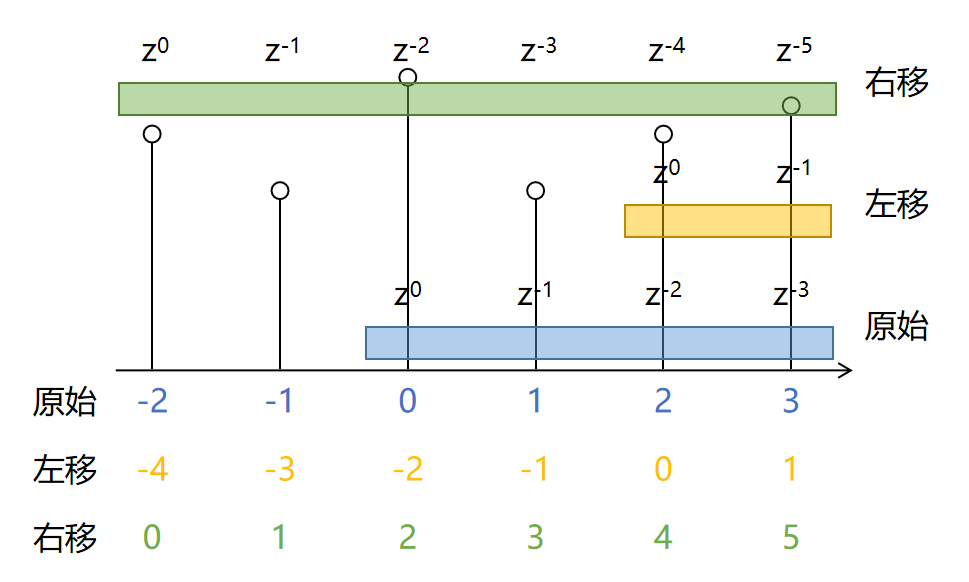
\includegraphics[scale=0.35]{Z变换时移.png}
                \end{figure}
        \end{itemize}
  \item 部分和:if $f[k]\leftrightharpoons F(z)$ \par
        \begin{itemize}[label=,left=3.5em]
          \item than $\sum_{i=-\infty}^{k}f[i]\rightleftharpoons{\frac{z}{z-1}F(z)}$
          \item 证明:$\sum_{i=-\infty}^{k}f[i]=f[k]*U[k]\rightleftharpoons{\frac{z}{z-1}F(z)}$
        \end{itemize}
  \item 初值/中值定理:$f[0]=\lim_{z\to +\infty}F(z)$
        \begin{itemize}[label=,left=6.9em]
          \item $f[\infty]=\lim_{z\to 1}\frac{z-1}{z}F(z)$
          \item 因果信号:$f[m]=\lim_{z\to +\infty}z^m F(z)$
        \end{itemize}
\end{enumerate}\par

\section{例题}
\begin{enumerate}[label=(\arabic*),itemindent=0pt,labelindent=\parindent,labelwidth=2em,labelsep=5pt,leftmargin=*]
  \item $\sum_{m=0}^{+\infty}\delta[k-mN]\rightleftharpoons\sum_{m=0}^{+\infty}z^{-mN}=\frac{1}{1-z^{-N}}=\frac{z^N}{z^N-1}\quad |z|>1$
  \item $a^kU[k]\rightleftharpoons F(\frac{z}{a})=\frac{z/a}{z/a-1}=\frac{z}{z-a}$
  \item $k\cdot U[k]$ \par
        解:\textcircled{1} \ 微分:$kU[k]\rightleftharpoons(-z)\frac{{\rm d}}{{\rm d}z}(\frac{z}{z-1})=(-z)\frac{(z-1)-z}{(z-1)^2}=\frac{z}{(z-1)^2}$
        \begin{itemize}[label=,left=1.5em]
          \item \textcircled{2} \ 卷积:$kU[k]=U[k]*U[k-1]\rightleftharpoons\frac{z}{z-1}\cdot\frac{z}{z-1}\cdot z^{-1}=\frac{z}{(z-1)^2}$
          \item \textcircled{3} \ 时移:令$f[k]=k\cdot U[k]$
                \begin{itemize}[label=,left=4.2em]
                  \item 则$f[k+1]=(k+1)U[k+1]=kU[k+1]+U[k+1]=f[k]+U[k]$
                  \item 等式两边进行Z变换:$zF(z)-zf[0]=F(z)+\frac{z}{z-1}$
                  \item 则$F(z)=\frac{z}{(z-1)^2}$
                \end{itemize}
        \end{itemize}
  \item $\sum_{i=0}^{k}a^i=\sum_{i=-\infty}^{k}a^iU[k]\rightleftharpoons\frac{z}{z-1}\cdot\frac{z}{z-a}$
\end{enumerate}\par

\section{逆Z变换}
\subsection{方法一}
$\sum_{i=1}^{M}a_iy[k=-m_i]=\sum_{i=1}^{N}b_if[k=-n_i]$ \par
$F(z)=\frac{b_mz^m+b_{m-1}z^{m-1}+\cdots+b_1z+b_0}{a_nz^n+a_{n-1}z^{n-1}+\cdots+a_1z+a_0}$
\begin{enumerate}[label=(\arabic*),itemindent=0pt,labelindent=\parindent,labelwidth=2em,labelsep=5pt,leftmargin=*]
  \item $m>n$,化简成$F(z)=\beta_1z^{m-n}+\beta_2z^{m-n-1}+\cdots+\beta_{i-1}z+\beta_i+F'(z)$的形式。
  \item $m\leqslant n$,$\frac{F(z)}{z}=\sum_{i=1}^{n}\frac{p_i}{z-z_i}$ \par
        例1:$F(z)=\frac{z+2}{2z^2-7z+3}$(单极点)\par
        \qquad 解:$\frac{F(z)}{z}=\frac{z+2}{2z(z-0.5)(z-3)}=\frac{p_1}{z}+\frac{p_2}{z-0.5}+\frac{p_3}{z-3}$ \par
        \qquad \qquad $p_1=\frac{F(z)}{z}z\big{|}_{z=0}=\frac{2}{3}$ \par
        \qquad \qquad $p_2=\frac{F(z)}{z}(z-0.5)\big{|}_{z=0.5}=\frac{z+2}{2z(z-3)}\big{|}_{z=0.5}=-1$ \par
        \qquad \qquad $p_3=\frac{F(z)}{z}(z-3)\big{|}_{z=3}=\frac{z+2}{2z(z-0.5)}\big{|}_{z=3}=\frac{1}{3}$ \par
        \qquad \qquad 则$\frac{F(z)}{z}=\frac{2}{3z}+(-1)\frac{1}{z-0.5}+\frac{1}{3}\frac{1}{z-3}$ \par
        \qquad \qquad 则$F(z)=\frac{2}{3}+(-1)\frac{z}{z-0.5}+\frac{1}{3}\frac{z}{z-3}$ \par
        \qquad \qquad 两边Z变换,得$f[k]=\frac{2}{3}\delta[k]+(-1)0.5^kU[k]+\frac{1}{3}3^kU[k]$ \par
        例2:$F(z)=\frac{z}{z^2+4}$(共轭双极点)\par
        \qquad 解:$\frac{F(z)}{z}=\frac{1}{(z+2j)(z-2j)}=\frac{k_1}{z+2j}+\frac{k_2}{z-2j}$ \par
        \qquad \qquad $k_1=\frac{F(z)}{z}(z+2j)\big{|}_{z=-2j}=\frac{1}{4j}=\frac{1}{4}e^{-j\frac{\pi}{2}}$ \par
        \qquad \qquad $k_2=\frac{1}{4}e^{j\frac{\pi}{2}}$ \par
        \qquad \qquad 代入后两边Z变换,得$f[k]=\frac{1}{4}e^{-j\frac{\pi}{2}}(2j)^kU[k]+\frac{1}{4}e^{j\frac{\pi}{2}}(-2j)^kU[k]$ \par
        \qquad \qquad \qquad \qquad \qquad \qquad \qquad \qquad \quad $=\frac{1}{2}2^k\cos[\frac{\pi}{2}k-\frac{\pi}{2}]U[k]$ \par
        例3:$F(z)=\frac{z^3+z^2}{(z-1)^3}$(多重极点)\par
        \qquad 解:$\frac{F(z)}{z}=\frac{z^2+z}{(z-1)^3}=\frac{k_{11}}{(z-1)^3}+\frac{k_{12}}{(z-1)^2}+\frac{k_{13}}{z-1}$ \par
        \qquad \qquad $k_{11}=\frac{1}{0!}\frac{F(z)}{z}(z-1)^3\big{|}_{z=1}=z^2+z\big{|}_{z=1}=2$ \par
        \qquad \qquad $k_{12}=\frac{1}{1!}\frac{{\rm d}}{{\rm d}z}(\frac{F(z)}{z}(z-1)^3)\big{|}_{z=1}=2z+1\big{|}_{z=1}=3$ \par
        \qquad \qquad $k_{13}=\frac{1}{2!}\frac{{\rm d}}{{\rm d}z^2}(\frac{F(z)}{z}(z-1)^3)\big{|}_{z=1}=1$ \par
        \qquad \qquad 则$F(z)=\frac{2z}{(z-1)^3}+\frac{3z}{(z-1)^2}+\frac{z}{z-1}$ \par
        \qquad \qquad 两边Z变换,得$f[k]=2k(k-1)U[k]+3kU[k]+U[k]$
\end{enumerate}\par
\subsection{方法二}
$F(z)=f[0]z^0+f[1]z^{-1}+f[2]z^{-2}+\cdots$ \par
例:$F(z)=\frac{z}{z^2-3z+2}=z^{-1}+3z^{-2}+7z^{-3}+\cdots$ \par
\qquad $f[k]=\{0,1,3,7,\cdots\}$
\begin{figure}[h]
  \qquad \qquad 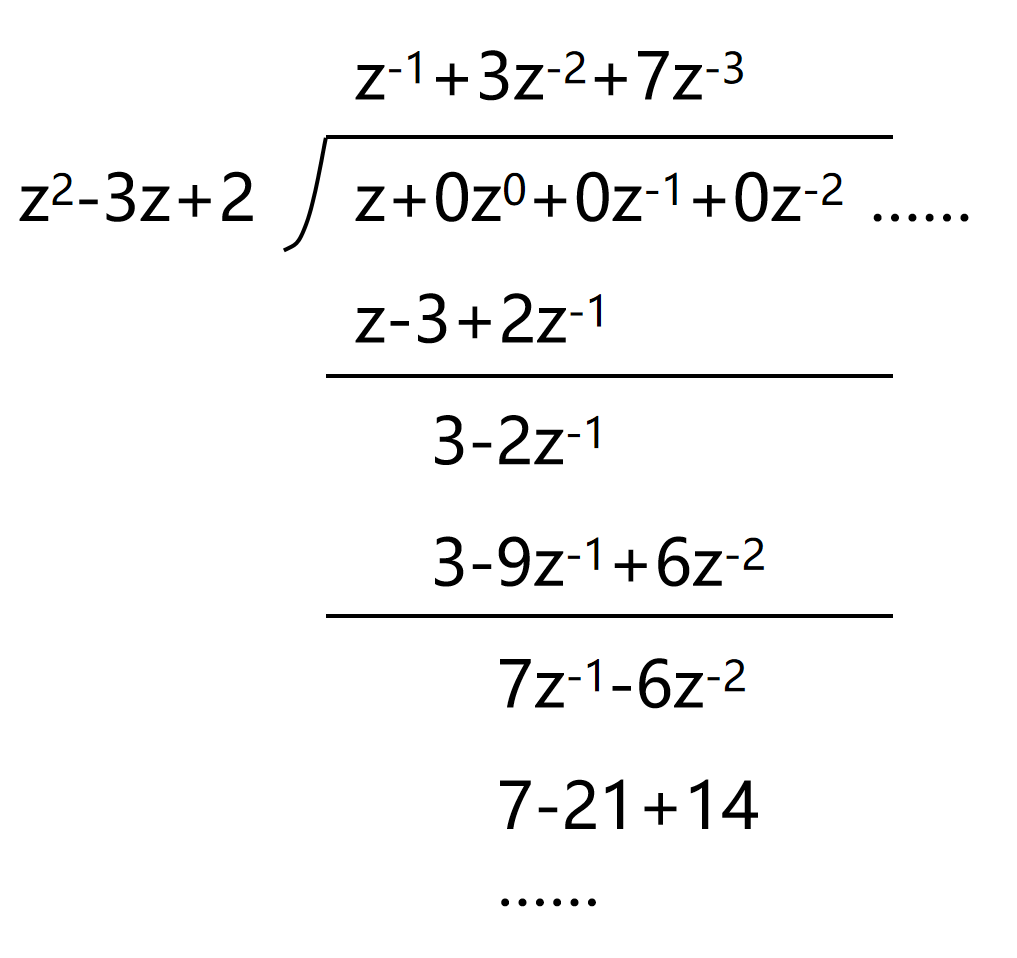
\includegraphics[scale=0.2]{逆Z变换方法二.png}
\end{figure}

\end{document}